\section{System Overview}

The core of the Action substrate is an object and experience layer running on the \textbf{AO compute network} \cite{Williams2024} and \textbf{Arweave} \cite{Williams2023} for persistence. Refer to Figure \ref{fig:system_overview} for a visual representation of the system.

\begin{figure}
  \centering
  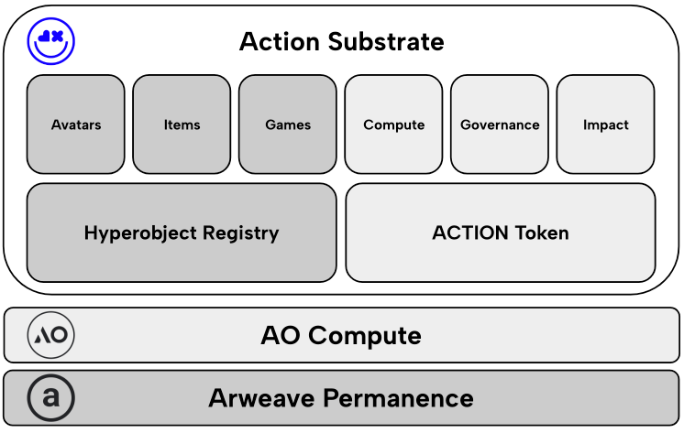
\includegraphics[width=0.95\columnwidth]{images/image3.png}
  \vspace{1em}
  \caption{ACTION runs on the AO Computer and Arweave, the global, permissionless hard drive.}
  \label{fig:system_overview}
\end{figure}

\textbf{Hyperobjects} are the foundational digital assets of the Action Substrate, serving as the building blocks for gameplay, commerce, and creativity across the ecosystem.

The \textbf{ACTION Token} allows for paying for Hyperobject creation and governance voting. Holder incentives are aligned around the expansion of robust, decentralized ecosystems built on game assets and engines. The main reason to acquire ACTION is to participate in the creation, gaming, or governance aspects, \textit{not} for speculative profit.

As the cost of creation continues to drop, Action reframes the value proposition around originality, collaboration, and community. By combining decentralized infrastructure with shared governance, it sets the stage for sustainable, vibrant communities, games and worlds built on the principles of creativity and ownership.

By integrating decentralized compute, AI-driven creation tools, and treasury-backed incentives controlled by the community, Action bridges the gap between digital innovation and real-world impact, supporting environmental and social initiatives through its governance mechanisms.

